\newpage
\section{動作実験}
%%%%%%%%%%%%%%%%%%%%%%%%%%%%%%%%%%%%%%%%%%%%%%%%%%%%%%%%%
\subsection{改良型細径羽状筋を備えたロボット}
3章2節と4章で述べた外骨格と羽状筋の設計方法と作製方法より開発した歩脚ロボットを図\ref{fig:kanirobot_new}に示す.
歩脚ロボットは長節,腕節,腕節,指節の4つの節で構成されている.
各節の内部には本研究で開発した改良型細径空圧羽状筋を備えている.

%%%%%%%%%%%%%%%%%%%%%%%%%%%%%%%%%%%%%%%%%%%%%%%%%%%%%%%%%
%
\begin{figure}[ht]
    \centering
    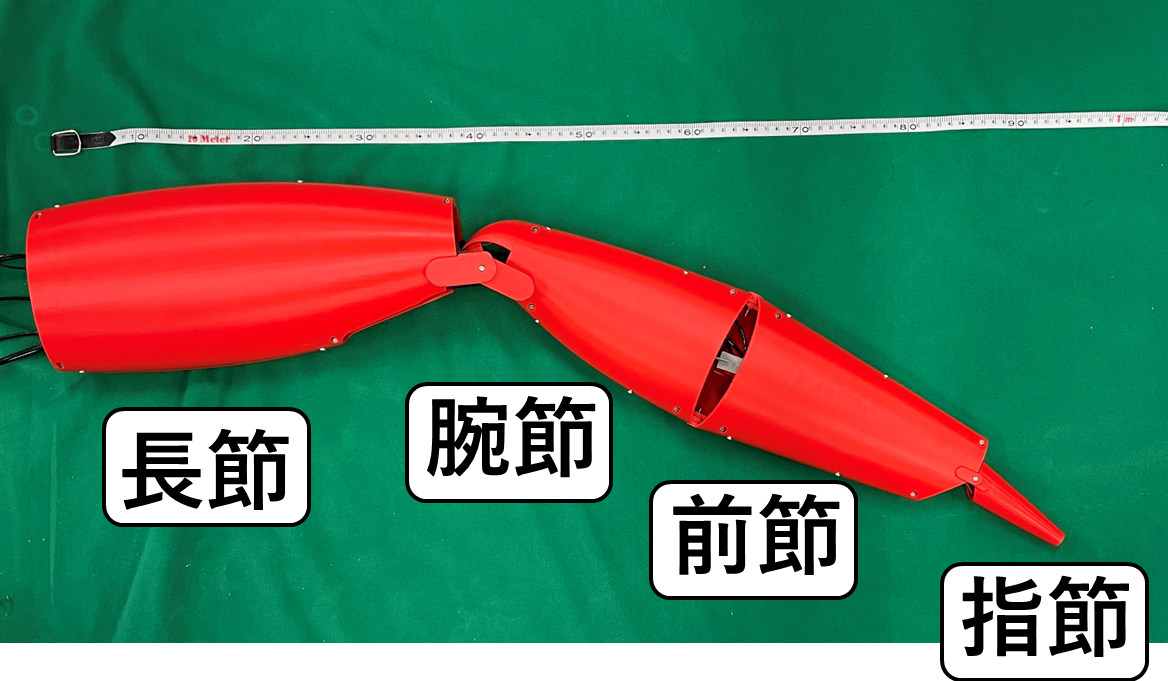
\includegraphics[scale=0.4]{image/jikki_2.png}
    \caption{本研究で作製した歩脚ロボット}
    \label{fig:kanirobot_new}
\end{figure}
%
\begin{figure}[t]
    \begin{minipage}{1\hsize}
      \centering
      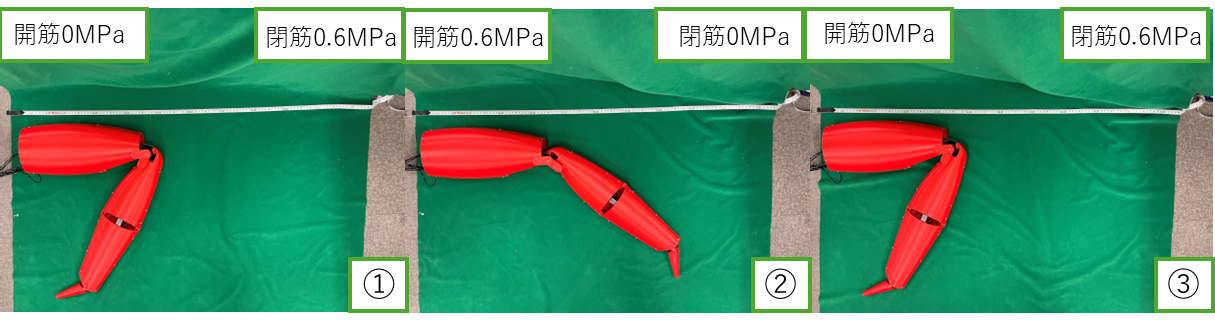
\includegraphics[scale=0.45]{image/chousetu-wansetu_edited.png}
      \vspace{-1mm}
      \subcaption{長節-腕節間の動作の様子}
      \label{fig:move_1}
    \end{minipage}
    %
    \begin{minipage}{1\hsize}
      \centering
      \vspace{3mm}
      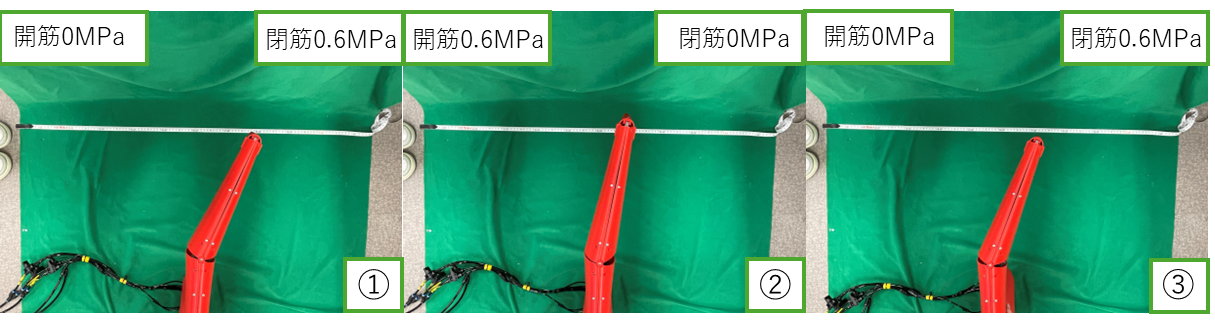
\includegraphics[scale=0.45]{image/wansetu-zensetu_edited.png}
      \subcaption{腕節-前節の動作の様子}
      \label{fig:move_2}
    \end{minipage}
    \begin{minipage}{1\hsize}
      \centering
      \vspace{3mm}
      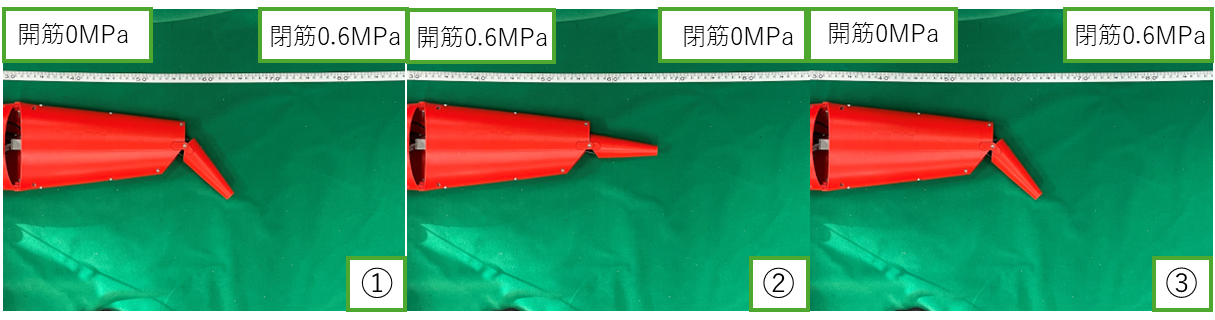
\includegraphics[scale=0.45]{image/zensetu-sisetu_edited.png}
      \subcaption{前節-指節の動作の様子}
      \label{fig:mone_3}
    \end{minipage}
\end{figure}
    %
%%%%%%%%%%%%%%%%%%%%%%%%%%%%%%%%%%%%%%%%%%%%%%%%%%%%%%%%%
\subsection{動作実験}

%%%%%%%%%%%%%%%%%%%%%%%%%%%%%%%%%%%%%%%%%%%%%%%%%%%%%%%%%
\subsection{実験結果}

%%%%%%%%%%%%%%%%%%%%%%%%%%%%%%%%%%%%%%%%%%%%%%%%%%%%%%%%%
\subsection{考察}
